\documentclass[pdf,bookmarks,colorlinks=true]{article}
\usepackage{multirow}
\usepackage{color,soul}
\usepackage{geometry}
\usepackage{amsthm}
\usepackage{hyperref}
\usepackage{graphicx}
\geometry{margin=0.5in}

\theoremstyle{definition}
\newtheorem{example}{Example}[section]

%opening
\title{Converting Ranges into Prefixes for Routers}
\author{Scot Anderson, Ph.D.}

\begin{document}

\maketitle

\section{Introduction}

In networking, students are often taught to calculate the set of longest-matching prefixes found in a routing table given a set of ranges or subnets with corresponding ports. This may seem trivial, but it is complicated by the fact that we may give a range of addresses instead of subnets. The basic steps in the algorithm, when given ranges, are as follows:

\begin{enumerate}
	\item Break each range up into legal subnets
	\item Join adjacent subnets that can be combined into a single subnet when they match the same link interface until no more combining can be done.
	\item If a link interface has more than one subnet, check if adjacent interface subnets would combine with it to create a single subnet encompassing both sets of subnets, call this A. If this is possible, replace the multiple subnets case (the one with the largest number of subnets) with A. Repeat until no more combinations can be made. Note once these two have been ``combined'' this way, they cannot participate in another combination. 
	\item List the prefixes, based on the subnets, in the list with their link interface as the final answer.   
\end{enumerate}

\section{Algorithm Step 1: Breaking down the ranges into subnets}

Given a range $[a, b]$, where $a, b \in \{x | x~matches~/ \textrm{\textasciicircum} [01]\{32\}\$/\}$ and $a < b$. Notice that the regular expression, $/ \textrm{\textasciicircum} [01]\{32\}\$/$, only matches a 32-bit binary string.\medskip

\textbf{Case 1}

Case 1 is the exit condition and occurs when $a$ and $b$ share a common prefix $p$ and $a = p||0*$\footnote{The symbol $||$ is commonly used for concatenation of strings. $0*$ or $[01]*$ means that the value 0 or (o or 1) can be repeated many times.} and $b = p||1*$. That is after the prefix, $a$ ends in all zeros and $b$ ends in all ones. Here $p$ is the one and only prefix needed to represent this range. Output $p$ and return.\medskip

\textbf{Case 2}

If Case 1 does not hold, then the following must hold $a = p||0||a_{end}*$ and $b = p||1||b_{end}*$ where $a_{end}, b_{end}$ are the strings of binary digits after the 0 and 1 respectively. Break this range up as follows:

Range 1: $[a_1, b_1] = [a, p||0||1*]$

Range 2: $[a_2, b_2] = [p||1||0*, b]$  

These ranges are contiguous and together represent the original range. The split location choice guarantees a split along a subnet boundary that has the potential to create the largest subnet in the range (if this is not obvious to the reader, consider that no smaller subnet mask can be created as it is limited by the prefix). The first range will always end at the  subnet boundary and the second range will begin on that same subnet boundary somewhere in the range. Because this split uses the shortest possible subnet mask, the split must take place in order to divide the range into legal subnets.

We finish Case 2 by running step 1 recursively on each Range 1 and Range 2 separately.

\begin{example}\label{ex:1}

Given the table of ranges below and the associated output interfaces, translate this into a longest-prefix-match routing table.\bigskip

\begin{center}
\begin{tabular}{|l|c|}\hline
	Destination Address Range &  Link Interface \\ \hline
	1100~0000~~1010~1000~~0000~1010~~0000~1100 & \multirow{2}{*}{0} \\
	1100~0000~~1010~1000~~0000~1010~~1111~1111 & \\ \hline
	1100~0000~~1010~1000~~0000~1011~~0000~0000 & \multirow{2}{*}{1} \\
	1100~0000~~1010~1000~~0000~1011~~0000~1111 & \\ \hline
	1100~0000~~1010~1000~~0000~1011~~0001~0000 & \multirow{2}{*}{2} \\
	1100~0000~~1010~1000~~0000~1011~~0001~1111 & ~\\ \hline 
	Otherwise & 3 \\ \hline
\end{tabular}\bigskip
\end{center}

Consider the base case where we have some prefix in common between the start and end of the range, denoted $[start, end]$

If start matches ``prefix0*'' and end matches ``prefix1*'', then the prefix for this range is ``prefix''. Ranges for Link interfaces 1 and 2 satisfy this condition, and we have a partially converted tables below.\bigskip

\begin{center}
\begin{tabular}{|l|c|}\hline
	Destination Address Range &  Link Interface \\ \hline
	1100~0000~~1010~1000~~0000~1010~~0000~1100 & \multirow{2}{*}{0} \\
	1100~0000~~1010~1000~~0000~1010~~1111~1111 & \\ \hline
	1100~0000~~1010~1000~~0000~1011~~0000 & 1 \\ \hline
	1100~0000~~1010~1000~~0000~1011~~0001 & 2 \\ \hline
	Otherwise & 3 \\ \hline
\end{tabular}\bigskip
\end{center}

We are going to split this range into two ranges at the first difference. Note: The first difference will always have a 0 in start and a 1 in end (highlighted below in yellow). The first range will always start with 0 and the second range will always start with 1. This makes two contiguous ranges and covers all of the original.\bigskip 

\begin{center}
	\begin{tabular}{|l|l|}\hline
		\multirow{2}{*}{Original} & 1100~0000~~1010~1000~~0000~1010~~\colorbox{yellow}{0}000~1100 \\
		& 1100~0000~~1010~1000~~0000~1010~~\colorbox{yellow}{1}111~1111 \\ \hline
		\multirow{2}{*}{First Range} & 1100~0000~~1010~1000~~0000~1010~~\colorbox{green}{0}000~1100 \\
		& 1100~0000~~1010~1000~~0000~1010~~\colorbox{green}{0}111~1111 \\ \hline
		\multirow{2}{*}{Second Range} & 1100~0000~~1010~1000~~0000~1010~~\colorbox{green}{1}000~0000 \\
		& 1100~0000~~1010~1000~~0000~1010~~\colorbox{green}{1}111~1111 \\ \hline
	\end{tabular}
\end{center}



In both cases we have extended our matching prefix by 1 bit (0 in the first range and 1 in the second range). The first range will need to be divided again, but the second range matches our base case and we can put out a prefix of: \textbf{1100~0000~~1010~1000~~0000~1010~~1}

Dividing up the first range will give us:\bigskip

\begin{center}
	\begin{tabular}{|l|l|}\hline
		\multirow{2}{*}{Original} & 1100~0000~~1010~1000~~0000~1010~~0\colorbox{yellow}{0}00~1100 \\
		& 1100~0000~~1010~1000~~0000~1010~~0\colorbox{yellow}{1}11~1111 \\ \hline
		\multirow{2}{*}{Second Range} & 1100~0000~~1010~1000~~0000~1010~~0\colorbox{green}{0}00~1100 \\
		& 1100~0000~~1010~1000~~0000~1010~~0\colorbox{green}{0}11~1111 \\ \hline
		\multirow{2}{*}{Second Range} & 1100~0000~~1010~1000~~0000~1010~~0\colorbox{green}{1}00~0000 \\
		& 1100~0000~~1010~1000~~0000~1010~~0\colorbox{green}{1}11~1111 \\ \hline
	\end{tabular}
\end{center}

Again the second range matches our base condition and we get a prefix of: \textbf{1100~0000~~1010~1000~~0000~1010~~01}. Breaking up the first one again gives us:\bigskip

\begin{center}
	\begin{tabular}{|l|l|}\hline
		\multirow{2}{*}{Original} & 1100~0000~~1010~1000~~0000~1010~~00\colorbox{yellow}{0}0~1100 \\
		& 1100~0000~~1010~1000~~0000~1010~~00\colorbox{yellow}{1}1~1111 \\ \hline
		\multirow{2}{*}{First Range} & 1100~0000~~1010~1000~~0000~1010~~00\colorbox{green}{0}0~1100 \\
		& 1100~0000~~1010~1000~~0000~1010~~00\colorbox{green}{0}1~1111 \\ \hline
		\multirow{2}{*}{First Range} & 1100~0000~~1010~1000~~0000~1010~~00\colorbox{green}{1}0~0000 \\
		& 1100~0000~~1010~1000~~0000~1010~~00\colorbox{green}{1}1~1111 \\ \hline
	\end{tabular}
\end{center}

Again the second range matches our base condition and we get a prefix of: \textbf{1100~0000~~1010~1000~~0000~1010~~001}. Breaking up the first one again gives us:\bigskip

\begin{center}
	\begin{tabular}{|l|l|}\hline
		\multirow{2}{*}{Original} & 1100~0000~~1010~1000~~0000~1010~~000\colorbox{yellow}{0}~1100 \\
		& 1100~0000~~1010~1000~~0000~1010~~000\colorbox{yellow}{1}~1111 \\ \hline
		\multirow{2}{*}{First Range} & 1100~0000~~1010~1000~~0000~1010~~000\colorbox{green}{0}~1100 \\
		& 1100~0000~~1010~1000~~0000~1010~~000\colorbox{green}{0}~1111 \\ \hline
		\multirow{2}{*}{Original} & 1100~0000~~1010~1000~~0000~1010~~000\colorbox{green}{1}~0000 \\
		& 1100~0000~~1010~1000~~0000~1010~~000\colorbox{green}{1}~1111 \\ \hline
	\end{tabular}
\end{center}

Our first range finally resolved to the base case condition. So the prefix is: \textbf{1100~0000~~1010~1000~~0000~1010~~0000~11}

Again the second range also matches our base case condition and we get a prefix of: \textbf{1100~0000~~1010~1000~~0000~1010~~0001}

Our set of prefixes looks like this:\bigskip

\begin{center}
	\begin{tabular}{|l|c|}\hline
		Destination Address Range &  Link Interface \\ \hline
		1100~0000~~1010~1000~~0000~1010~~1 & \multirow{4}{*}{0}\\
		1100~0000~~1010~1000~~0000~1010~~01 & \\
		1100~0000~~1010~1000~~0000~1010~~001 & \\
		1100~0000~~1010~1000~~0000~1010~~0001 & \\
		1100~0000~~1010~1000~~0000~1010~~0000~11 & \\ \hline
		1100~0000~~1010~1000~~0000~1011~~0000 & 1\\ \hline
		1100~0000~~1010~1000~~0000~1011~~0001 & 2\\ \hline 
		Otherwise & 3 \\ \hline
	\end{tabular}\bigskip
\end{center}

\end{example}

\section{Algorithm Step 2: Joining adjacent subnets ... or Reverse subnetting}

When we learned subnetting, we broke a range into two halves. When we are aggregating routes we do the reverse and combine two adjacent prefixes that can be combined into a subnet with a shorter mask. In this step we only aggregate routes that are using the same port. 

If there was only one range assigned to a port, you should satisfy yourself that there can be no route aggregation for the port. I.e. if you could combine them here, we would not have split them in the previous step. 

If there were multiple ranges assigned to a port (very possible if we are routing to another organization), then we may be able to aggregate routes similar to how we broke them up in the first step. 

\begin{example}\label{ex:2}
	\begin{figure}[hb]
		\centering
		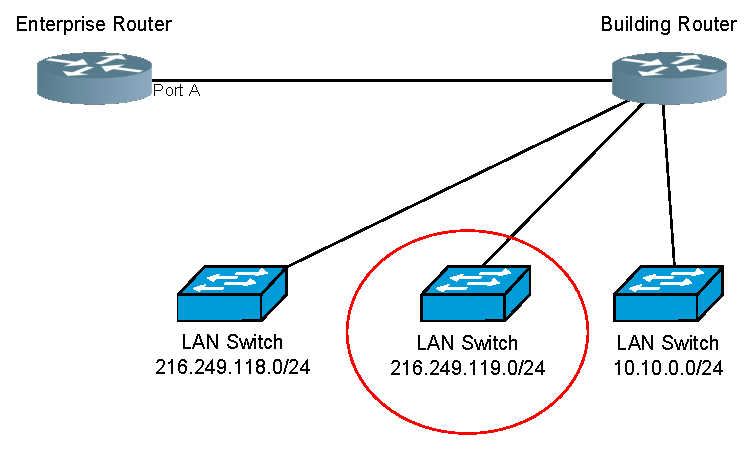
\includegraphics[width=0.6\linewidth]{example2.pdf}
		\caption{Enterprise Routes}
		\label{fig:router_config}
	\end{figure}
	
	Suppose at some time in the past we allocated 216.249.118.0/24 and 10.10.0.0/24 to a building router from our enterprise router. The building router then routes those prefixes to switches (Local Area Networks). Figure~\ref{fig:router_config} shows an added subnet to the Building Router shown in the red circle. At the enterprise router level, we now have two route prefixes both going to the Building router: 
	\begin{center}
		\begin{tabular}{|l|c|}\hline
			Prefixes & Link Interface \\ \hline
			1101~1000~~1111~1001~~0111~0110 & A \\
			1101~1000~~1111~1001~~0111~0111 & A \\ \hline
		\end{tabular}
	\end{center}
	These prefixes are identical until the last bit, hence they are contiguous ranges, the same size and can be combined to have the same prefix. Namely:  
	\begin{center}
		\begin{tabular}{|l|c|}\hline
			Prefixes & Link Interface \\ \hline
			1101 1000  1111 1001  0111 011 & A \\ \hline
		\end{tabular}
	\end{center}
	
\end{example}

\section{Algorithm Step 3: Subnet Aggregation to achieve minimal prefixes using Longest Prefix}

In some cases we may not immediately see a way to join two prefixes because they point to different ports. Consider Example~\ref{ex:1}. Every prefix starts with 192.168.10 and is broken somewhere in the last byte. Consider the tree of these shown in Figure~\ref{fig:prefix_tree}. Everything but the two blue subnets are assigned to Port 0. It would be awfully nice if we could somehow reduce the number of prefixes going to Port 0... and we can! 
\begin{figure}[ht]
	\centering
	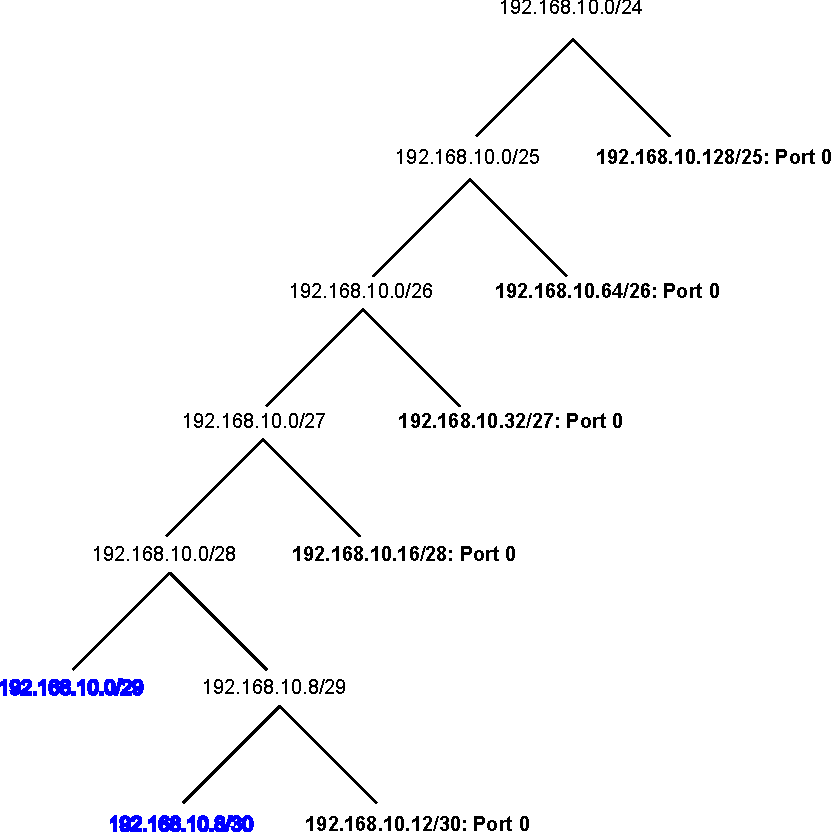
\includegraphics[width=0.6\linewidth]{example1_tree.pdf}
	\caption{Prefixes as subnet tree.}
	\label{fig:prefix_tree}
\end{figure}

Logic dictates that there are only two possibilities. (1) The ISP who assigned me IPs has retained these subnets or, (2) they belong to our network and we have not assigned them. In the first case, it would make sense to route these to our ISP out port 3. If I am holding them for some network that will soon be assigned, I could just route these subnets to /dev/null (in Linux parlance). Suppose that these two subnets are assigned to a new Link interface called port 4. We could use the longest matching prefix aggregate our subnets as follows:

\begin{center}
	\begin{tabular}{|l|c|}\hline
		Destination Address Range &  Link Interface \\ \hline
		1100~0000~~1010~1000~~0000~1010 & 0 \\ \hline
		1100~0000~~1010~1000~~0000~1011~~0000 & 1\\ \hline
		1100~0000~~1010~1000~~0000~1011~~0001 & 2\\ \hline 
		Otherwise & 3 \\ \hline
		1100~0000~~1010~1000~~0000~1010~~0000~0 & \multirow{2}{*}{4} \\
		1100~0000~~1010~1000~~0000~1010~~0000 10 & \\ \hline
	\end{tabular}\bigskip
\end{center}

\section{Summary}

We have shown an algorithm that is capable of creating minimal, longest prefix matching routing tables. The first step has been programmed by your professor and is available on \href{https://github.com/scotpatti/Range2LongestPrefix}{github}.

\end{document}
